\section{Middlware, communications patterns and their applications}

In a distributed system, we view middleware as one or multiple applications that homogenize and simplifies the communication and integration between nodes. It is suitable to link systems of various origin and to institute so-called "plumbing", but may add complexity and extra cost to the design and additional overhead, as data from the application-layer (user-space) has to traverse a extra layer of middleware protocols before being put on a wire or broadcasted to its destination. This is seen in figure \ref{fig:middleware}. 

\begin{figure}[h!]\label{}
	\centering
	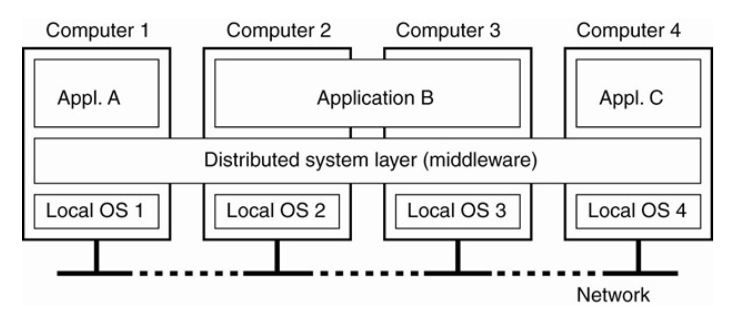
\includegraphics[scale=0.5]{middleware/middlewaredist.png}
	\caption{Middleware in a distributed system, situtaed between the application layer and the internal part of the local operating system.}
	\label{fig:middleware}
\end{figure}

\noindent Three examples of modern middleware is the open-source message-broker RabbitMQ, the web-server specification OWIN for .NET and the DDS standard, which we will discuss in the next section. RabbitMQ provides a simple client interface to a broker, that can exchange messages in a distributed system. We define it as middleware because it manages connectivity and message passing among two systems. OWIN defines a interface between .NET web servers and applications, meaning all the layers between a public API and the actual web server. This includes deserializing the HTTP request,   invoking authentication modules and generating response data. Whichever middleware application we consider, they offer various traits in a distributed system. We look at three key ones, space, time and flow decoupling:

\noindent \textbf{Space}: Producers and consumers do not know each-other and no direct link exist.

\noindent \textbf{Time}: Communication is asynchronous. A producer or consumer does not have to wait on the counterpart.

\noindent \textbf{Flow}: The data production and consumption does not reside in the main flow of the producer or the consumer, i.e. they have additional threads or loops to handle calls.

\noindent Decoupling removes the implied dependency between producer and consumer, when communications occur. These decoupling traits are important when examining middleware applications and its communication-patterns. To quickly review just a few of these, we provide a short list and address their traits:

\begin{itemize}
	\item Remote procedure call (RPC): Used to call services on other nodes directly and make them look local to the particular service. Does not provide space or time decoupling, as call is point-to-point and synchronous. Used in for example Java RMI.
	\item SQL orientation: Used to mask underlying SQL procedure calls and translate database instructions into higher-level code. Synchronous in time and often use a direct database connection string, i.e. no time or space decoupling.
	\item Asynchronous Messaging: Modern web applications use this in protocols like AJAX. This pattern is time and flow decoupled, as requested are executed in separate threads and no blocking is introduced.
	\item Publish-subscribe: Messages between nodes are published to topics based on type and sent to a centralized or distributed broker, which forwards messages to specific nodes, that have subscribe to that message type. This pattern provides space, time and flow decoupling.
\end{itemize}

\noindent The publish-subscriber pattern provides all of three mentioned traits and figure \ref{fig:pubsub} illustrates how a central broker (EventService) can use this pattern to archive space, time and flow decoupling. It works by subscribers registering at the broker for certain events or type of information by calling subscribe(). A publisher then publishes a message to the broker using notify(). If any subscribers have subscribed to that particular type of message or data, they have notified by the broker with notify().

\begin{figure}[h!]\label{}
	\centering
	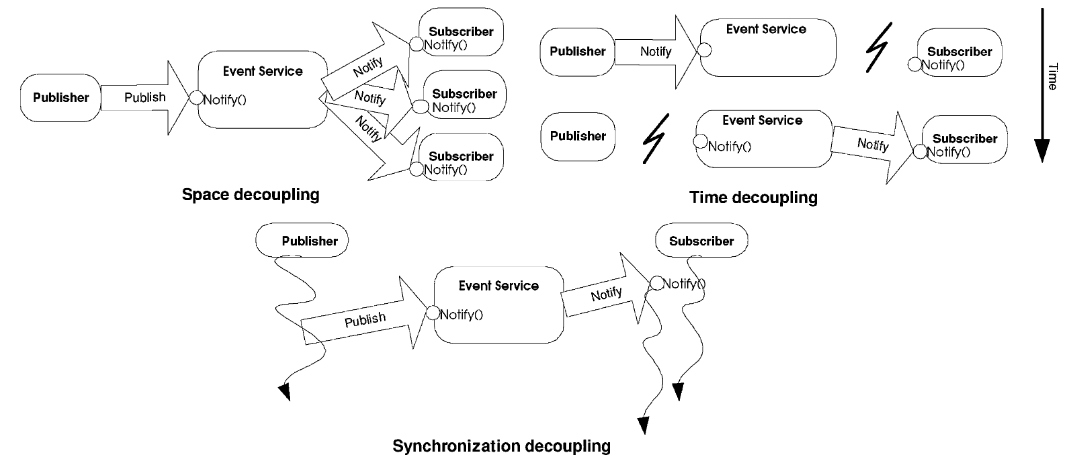
\includegraphics[scale=0.6]{middleware/pubsub.png}
	\caption{The publish-subscribe pattern archives space, time and flow decoupling.}
	\label{fig:pubsub}
\end{figure}